% !TeX root = ../main.tex
% Add the above to each chapter to make compiling the PDF easier in some editors.

\chapter{User Study}\label{chapter:userstudy}
The effectiveness of teleoperation interfaces must be evaluated through rigorous user studies to ensure they meet the requirements for situational awareness, cognitive load management, and overall usability. This chapter details our comprehensive user study comparing the Separate View and Integrated View approaches for perception modification tasks.

Our study design focuses on three key aspects identified in the literature review: situational awareness measured through SAGAT, cognitive workload assessed using NASA-TLX, and feature completeness evaluated through expert feedback. To ensure ecological validity and relevance to our target users, we developed a custom simulation environment based on Munich's road infrastructure, moving away from the US-centric scenarios typical in CARLA simulations.

The study incorporates multiple scenarios designed to test different aspects of perception modification tasks, with particular attention to situations where autonomous vehicles commonly require human intervention. These scenarios were carefully crafted to evaluate both interfaces under comparable conditions while maintaining realistic challenges faced in urban environments.

This chapter begins by a detailed explanation of the study design, including scenario selection and questionnaire development. We then outline the preparation process, including map creation, scenario recording and video creation, and conclude with a discussion of our analysis techniques for evaluating the collected data.

\section{Study Design}


\subsection{Scenarios}
The scenarios for the user study were designed to evaluate the effectiveness of the Separate View and Integrated View interfaces in supporting perception modification tasks. The goal was to create a diverse set of scenarios that reflect real-world challenges in autonomous driving, focusing on three main categories: modification of objects, modification of drivable space, and unsolvable scenarios. Each category includes multiple variants to ensure comprehensive testing across different situations.
\subsubsection{Modification of Objects}
These scenarios involve correcting misperceptions related to objects detected by the autonomous vehicle's perception system. They test the operator's ability to identify and modify object-related errors in detection, classification, prediction, and position/size:
\begin{table}[h!]
    \centering
    \begin{tabular}{|p{6cm}|p{7.8cm}|}
    \hline
    \textbf{Scenario} & \textbf{Description} \\
    \hline
    Water pond detected as an object & Tests the operator's ability to identify false-positive detections. \\ \hline
    Leaves on the road misclassified & Evaluates how operators handle misclassification of small objects. \\ \hline
    Carton on the road misclassified & Similar to the leaves scenario but with a different object type. \\ \hline
    Pedestrians at a crosswalk not intending to cross & Challenges operators to correct prediction errors. \\ \hline
    Second-row parker detected as a dynamic vehicle & Tests handling of incorrect dynamic predictions. \\ \hline
    Tree branches leaning onto the road detected as blocking objects & Wrong classification of the tree branches. \\ \hline
    Crowd of pedestrians on a sidewalk & Tests operator handling of large groups of pedestrians with position errors in the detection. \\ \hline
    \end{tabular}
    \caption{Scenarios for object modification tasks}
    \label{table:scenariosobjectmodification}
    \end{table}
\subsubsection{Modification of Drivable Space}
These scenarios test how well operators can modify errors in the perceived drivable area:
\begin{table}[h!]
    \centering
    \begin{tabular}{|p{6cm}|p{7.8cm}|}
    \hline
    \textbf{Scenario} & \textbf{Description} \\
    \hline
    Construction site (two variants) & Evaluates operators' ability to adjust drivable space around construction zones. \\ \hline
    Traffic island detected as an undefined object & Tests corrections for drivable area misinterpretations. \\ \hline
    \end{tabular}
    \caption{Scenarios for drivable area modification tasks}
    \label{table:scenariosdrivablemodification}
    \end{table}

\subsubsection{Unsolvable Scenarios}
These scenarios represent edge cases where no modifications can resolve the issue. They test how operators handle situations beyond their control:

\begin{table}[h!]
    \centering
    \begin{tabular}{|p{6cm}|p{7.8cm}|}
    \hline
    \textbf{Scenario} & \textbf{Description} \\
    \hline
    Completely occluded traffic light blocked by a truck & Evaluates decision-making when critical information is unavailable. \\ \hline
    Blocked one-way street (two variants) & Tests operator responses to unresolvable roadblocks. \\ \hline
    \end{tabular}
    \caption{Scenarios for unsolvable tasks}
    \label{table:scenariosunsolvable}
    \end{table}

The scenarios were selected from a subset defined in El Alami's thesis \cite{yassinethesis}, focusing on those most relevant to perception modification tasks. Each scenario was designed to ensure consistency across tests while remaining challenging enough to evaluate operator performance effectively.

\subsection{Questionnaire}

\section{Study Preparation}

\subsection{Map creation for CARLA}\label{section:mapcreationforcarla}
To ensure the ecological validity of our user study and provide a realistic simulation environment, we developed a custom map for CARLA based on the Gärtnerplatz square in Munich, Germany. This section describes the map creation process, which involved replicating the real-world location as closely as possible while adapting it to the capabilities of the CARLA simulator.
\subsubsection*{Pipeline Overview}
\begin{figure}
    \centering
    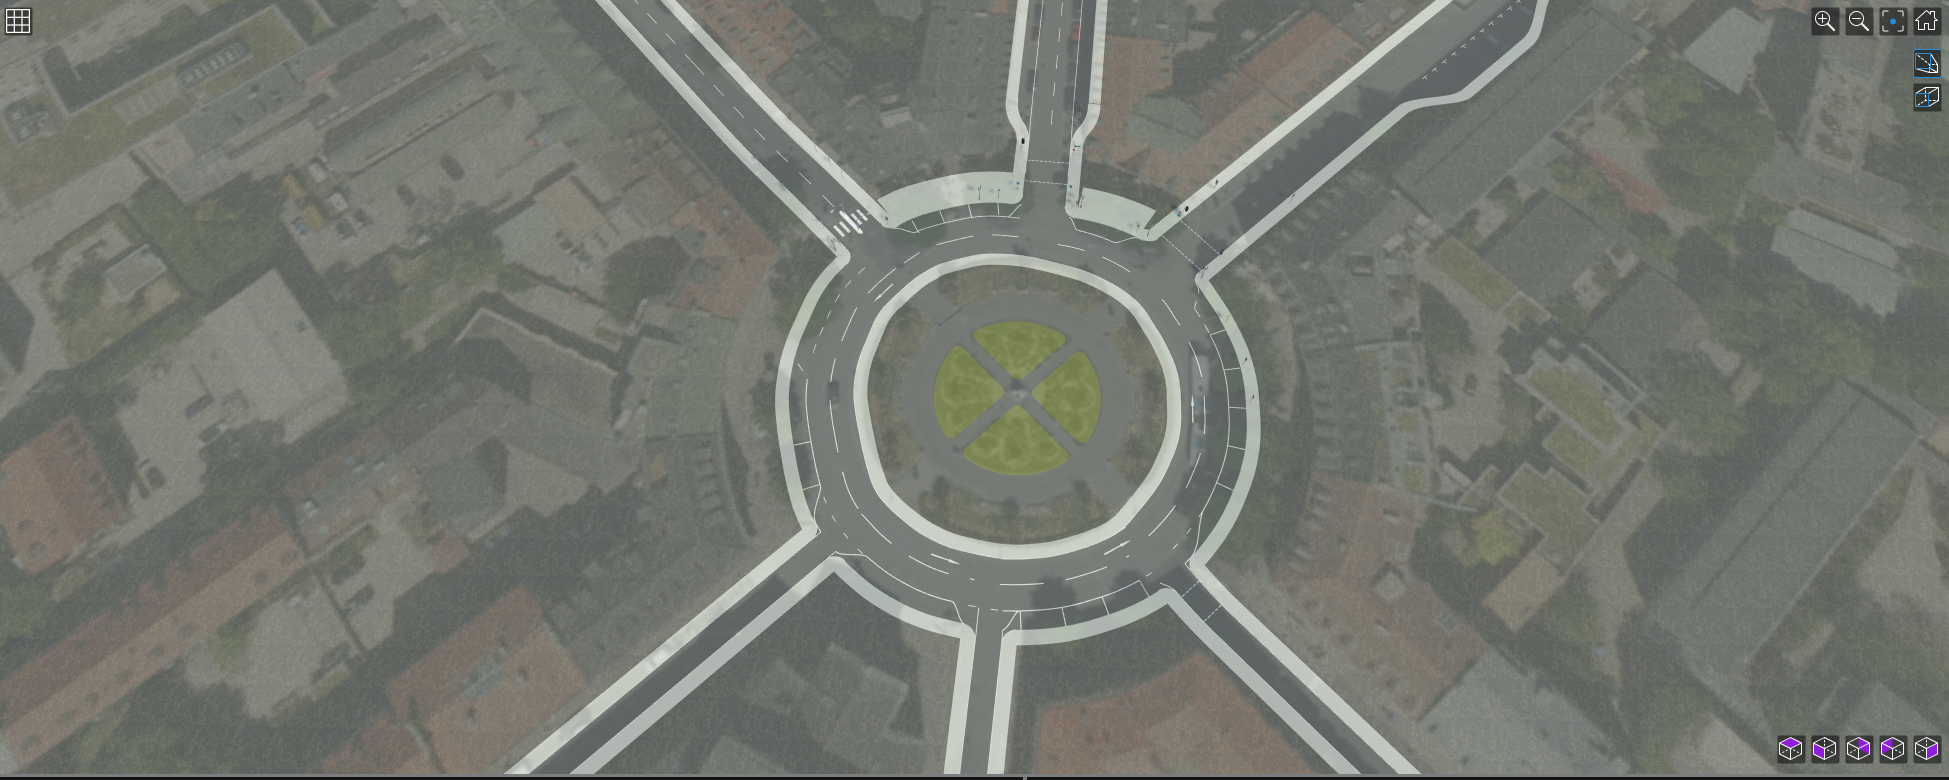
\includegraphics[width=\textwidth]{figures/roadrunner.png}
    \caption{Road network design of Gärtnerplatz in MathWorks RoadRunner}
    \label{fig:roadrunner}
\end{figure}
The map creation process followed a structured pipeline:
\begin{enumerate}
    \item Road Network Creation: Using MathWorks RoadRunner, we designed the road network based on satellite data obtained from the Geoportal Bayern \cite{geoportal_bayern}. The road network included all major features of Gärtnerplatz, such as the six-way roundabout, one-way roads, two-way roads with traffic islands, and traffic lights at intersections. Regulatory elements like crosswalks, traffic signs, and lane markings were added to align with real-world traffic rules. The results can be seen in Result can be seen in \ref{fig:roadrunner}.
    \item Export to OpenDRIVE: The road network and regulatory elements were exported in OpenDRIVE format using RoadRunner's export tools \cite{mathworks_roadrunner}.
    \item Import into Unreal Engine: The OpenDRIVE file and associated assets were imported into Unreal Engine using CARLA's RoadRunner import plugin \cite{carla_map_import}. This step included setting up the road geometry, lane configurations, and traffic rules within CARLA's simulation environment.
    \item Environment Art: Additional environment details, such as buildings, vegetation, and textures, were created in Unreal Engine using CARLA's default asset set. The visual elements were designed to replicate the appearance of Gärtnerplatz as closely as possible.
\end{enumerate}

\begin{figure}[h]
    \centering
    \begin{subfigure}{\textwidth}
        \centering
        \includegraphics[width=\textwidth, trim=0 200pt 0 200pt, clip]{figures/sim_top.png}
        \caption{Top view of the simulation environment}
        \label{fig:sim_top}
    \end{subfigure}
    \begin{subfigure}{\textwidth}
        \centering
        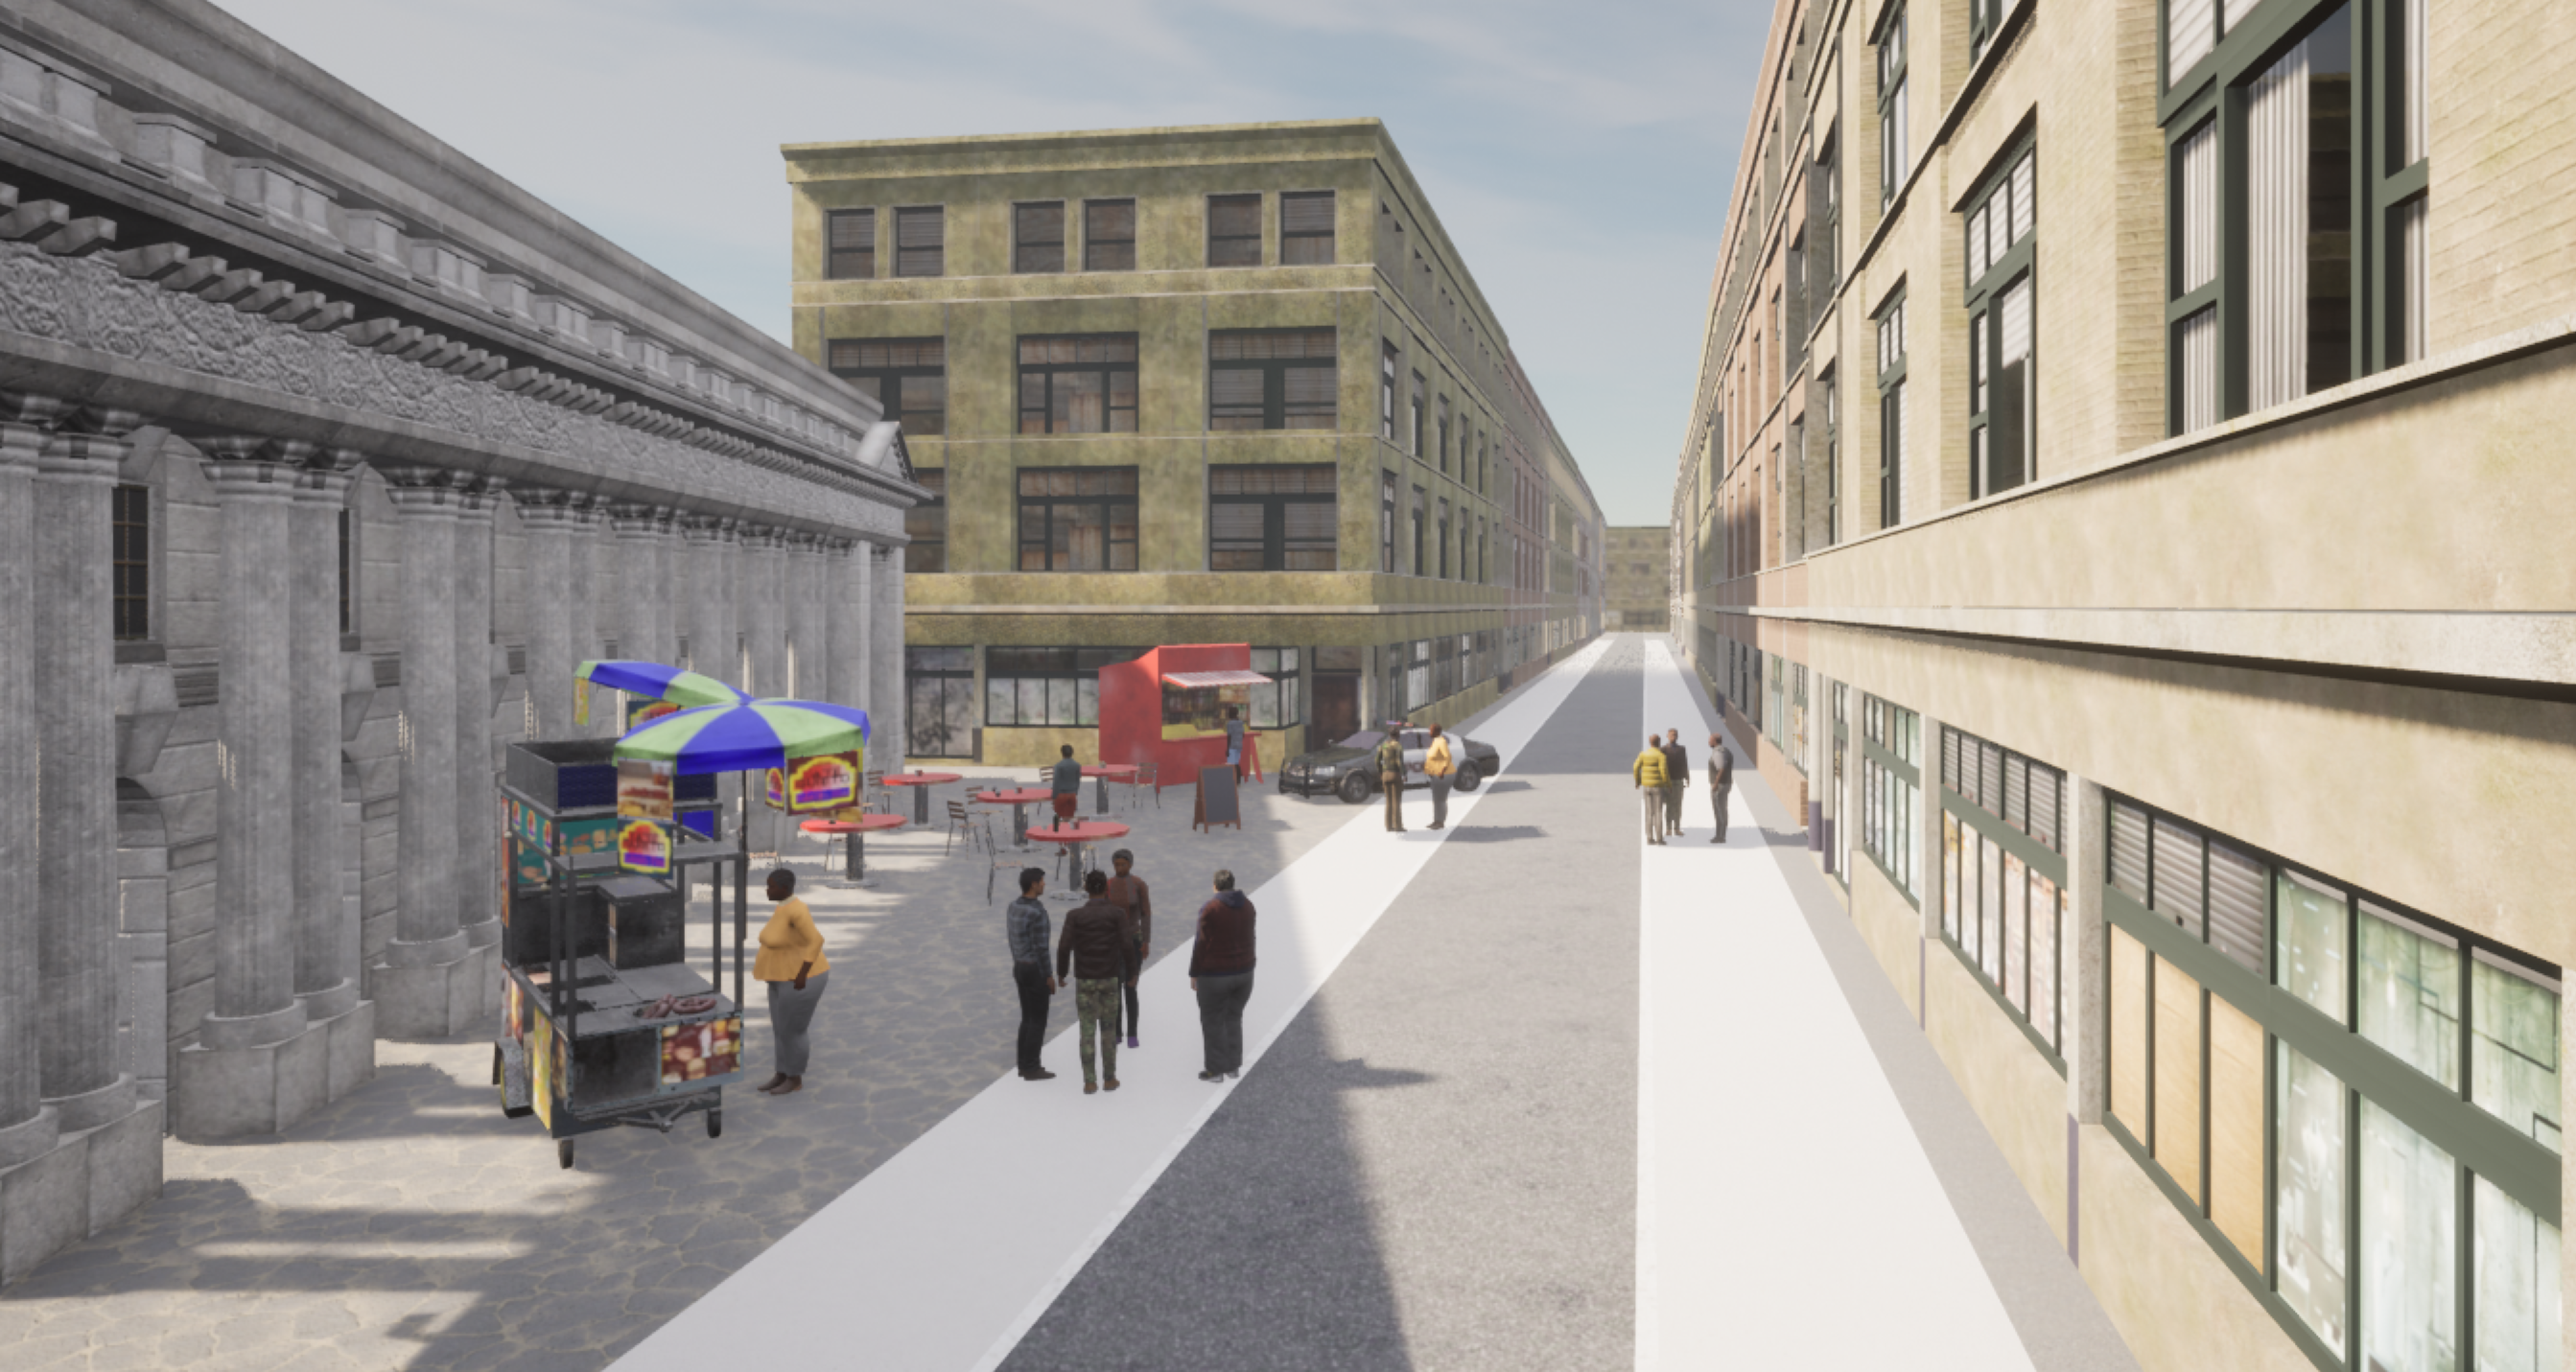
\includegraphics[width=\textwidth, trim=0 200pt 0 200pt, clip]{figures/sim_crowd.png}
        \caption{Environment is detailed to provide a dynamic city look}
        \label{fig:sim_crowd}
    \end{subfigure}
    \begin{subfigure}{\textwidth}
        \centering
        \includegraphics[width=\textwidth, trim=0 200pt 0 200pt, clip]{figures/sim_signs.png}
        \caption{Local traffic signs are used in their real-world locations}
        \label{fig:sim_signs}
    \end{subfigure}
    \caption{Simulation environment based on Gärtnerplatz square}
    \label{fig:simulation}
\end{figure}
\FloatBarrier
\subsubsection*{Real-World Location Selection}
The Gärtnerplatz square was selected due to its unique traffic layout and diverse road types:
\begin{itemize}
    \item A six-way roundabout at the center
    \item One-way roads leading in different directions
    \item Two-way roads with traffic islands and signalized intersections
    \item A central square surrounded by buildings, creating a visually complex and busy scene
\end{itemize}

Satellite imagery from Geoportal Bayern \cite{geoportal_bayern} served as the basis for road layout design. Google Maps' Street View feature was used to identify traffic signs, building types, and vegetation patterns. These references ensured that the map accurately reflected real-world conditions while remaining computationally efficient for simulation.

\subsubsection*{Challenges and Adaptations}
While we aimed to replicate Gärtnerplatz accurately, certain adaptations were necessary due to computational constraints:
\begin{itemize}
    \item Simplified building models and vegetation to reduce rendering overhead
    \item Adjustments to road curvature and lane widths to meet CARLA's simulation requirements
    \item Replacement of some real-world assets with CARLA's default textures
\end{itemize}

These adaptations ensured that the map remained computationally efficient while preserving key features relevant to our user study scenarios.
By creating a map tailored to our study's requirements, we provided participants with a realistic yet controlled simulation environment for evaluating teleoperation interfaces.
\subsection{Scenario Recording}
\subsection{Video Creation}
\section{Analysis Techniques}
